%\chapter{Interaction of Particles with Matter Part-II - Radiation}
%\label{matter_radiation_interaction} % Always give a unique label

\section{The Cerenkov Radiation}
Let's consider a particle travelling through a medium with a
refraction index $n$ and a velocity $\beta c$. It is possible that the
particle travels at a speed which is higher than the one of the light
in that medium, which is $c/n$, if
\[\beta > \frac{1}{n}.\]
This phenomenon is usually associated with the emission of a radiation
by the material (\emph{Cerenkov radiation}) which is represented in
figure \ref{fig:passRadMat14}\footnote{A nice animation which illustrates the effect is available at  \url{https://upload.wikimedia.org/wikipedia/commons/8/87/Cherenkov_radiation-animation.gif}.}. Atoms of the material are polarised by
the motion of the particle and release radiation in spherical
waves. The envelope of these waves is a plane wave emitted at a
certain angle $\theta_c$. If the distance covered by the light
emission in a time $t$ is equal to the distance covered by the
particle, then
\[\beta c t \cos\theta_c = \frac{ct}{n}\]
which gives:
\[\cos\theta_c = \frac{1}{n\beta}\]

\begin{figure}
  \centering 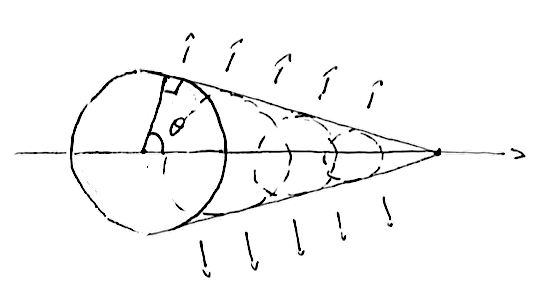
\includegraphics[width=0.5\textwidth]{passRadMat14}
  \caption{Illustration of the Cerenkov Radiation and its emission angle $\theta$.}
  \label{fig:passRadMat14}
\end{figure}

The emitted energy per unit of photon frequency $\omega$ by a particle of charge $ze$
can be computed within classical electrodynamics, and corresponds to
\begin{eqnarray*}
  \frac{d^2E}{dx d\omega} &=& \frac{z^2e^2}{4\pi \epsilon_0}\frac{\omega}{c^2}\qq{1-\frac{1}{\beta^2n^2(\omega)}}  \\
                          &=& z^2\frac{\alpha\hslash\omega}{c}\sin^2(\theta_c(\omega)),
\end{eqnarray*}
where $\alpha=\frac{e^2}{4\pi\epsilon_0\hslash c}=\frac{1}{137}$ is the fine structure constant. 
A typical Cerenkov detector is sensitive (and transparent) only to some part of the photon spectrum. The number of photons with energy equal to $\hslash\omega$ can be written as
\[\frac{d^2n}{dxd\omega}=\frac{z^2\alpha}{c}\sin^2\theta_c(\omega),\]
and we want to integrate it in an interval of visible frequencies. We obtain
\begin{eqnarray*}
  \frac{dn}{dx}&=&\frac{z^2\alpha}{c}\int_{\Delta\omega} \sin^2\theta_c(\omega)d\omega  \\
               &\simeq& \frac{z^2\alpha}{c}\avg{\sin^2\theta_c}\Delta\omega,
\end{eqnarray*}
which for a typical range of photon spectrum $\hslash\omega\approx\SI{2}{eV}$ corresponds to
\[\avg{\der{n}{x}} \sim 700\ \text{photons}\ \centi\meter^{-1} \times
  z^2\sin^2\theta_c\] Cerenkov emission does not contribute to the
energy loss for a particle, since its intensity is $10^{3}$ times less
than ionisation energy loss, this is rather intuitive since this
emission is due to a polarisation effect. Typically, Cerenkov photon
have an energy of $4\,\electronvolt$, and the average energy loss is
around $2\,\kilo\electronvolt$.

\begin{figure}
  \centering 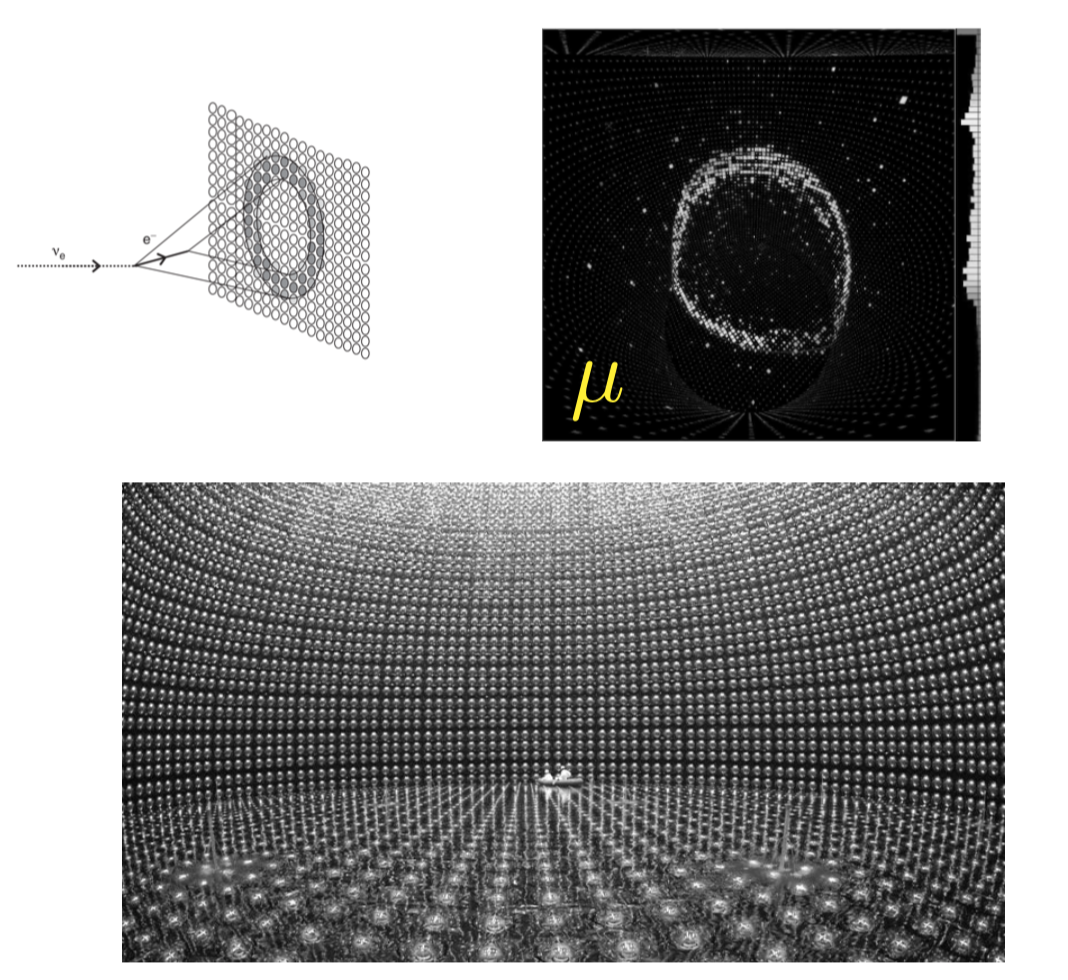
\includegraphics[width=\textwidth]{passRadMat15}
  \caption{Top left: Cerenkov ring due to the emission of Cerenkov
    radiation. Bottom: Super Kamiokande is a detector which is
    based on Cerenkov radiation detection, the radiator material is
    water ($50\times10^3 \kilo\gram$) and it is equipped with 11k
    light detectors. Top right: an image of a reconstructed Cerenkov ring produced by a muon in the Super Kamiokande detector.}
  \label{fig:passRadMat15}
\end{figure}


\section{Multiple Scattering}
We have computed the Rutherford differential cross section in Chapter~\ref{Scattering-1}, Eq.~\eqref{eq:rutherford}, which describes the interaction between a particle of charge $z$ and an atomic nucleus with atomic number $Z$, as a function of the scattering angle $\theta$:
\[
 \frac{d\sigma}{d\Omega} =\left( \frac{zZe^2}{16 \pi \varepsilon_0 E_k} \right)^2 \times \frac{1}{\sin^4 \dfrac{\theta}{2}}.
\]
Here we used $E_k$ to denote the kinetic energy of the charged particle.

From the Rutherford formulation it is clear that the cross section diverges at small angles,
\[\lim_{\theta\to 0}\der{\sigma}{\Omega} = \infty. \]
This implies that the average scattering angle is $\avg{\theta} = 0$. 

Under the hypothesis that a particle undergoes multiple independent scatterings in a material, it is reasonable to assume the mean scattering angle to be Gaussian--distributed. How much will the standard deviation (or the variance) of this Gaussian be? This is the relevant experimental quantity, as a beam of particles traveling in matter will somehow be ``spread'' by that amount.

In an element of solid angle $d\Omega = 2\pi \sin \theta d\theta \approx 2 \pi \theta d\theta$, the number of collisions can be expressed then as a function of the kinetic energy, which can be written as $E_k = pv/2$:
\begin{eqnarray*}
  d^2n &=& \frac{\mathcal{N}_A\rho}{A} d\sigma dx\\
  &=& \frac{\mathcal{N}_A\rho}{A} \frac{d\sigma}{d\Omega} 2 \pi \theta d\theta dx\\
  &=& 8\pi \frac{\mathcal{N}_A\rho}{A} r_e^2 z^2Z^2 \frac{(m_ec^2)^2}{p^2v^2}\frac{\theta d\theta dx}{\theta^4},
\end{eqnarray*}
in which we used the complete Rutherford cross section computed in Eq.~\ref{eq:rutherford} in the approximation of small angles.

Given that the average scattering angle is zero, the variance of the scattering angle is simply the expectation value of the square of the scattering angle,
\begin{eqnarray*}
  \theta^2_s &=& \int \theta^2  \frac{d^2n}{d\theta dx}d\theta \\
                   &=& 8\pi r_e^2 \frac{\mathcal{N}_A \rho}{A} z^2 Z^2 \frac{\rr{m_ec^2}^2}{p^2v^2}\int\frac{d\theta}{\theta}\\
                   &=& 8\pi r_e^2 \frac{\mathcal{N}_A \rho}{A} z^2 Z^2 \frac{\rr{m_ec^2}^2}{p^2v^2} \ln\frac{\theta_{\max}}{\theta_{\min}}
\end{eqnarray*}

From here we can use again the relation between the impact parameter $b$ and the scattering angle $\theta$ of Eq.~\eqref{eq:ImpactParameterR} derived in Chapter~\ref{Scattering-1}, which can be written in terms of $r_e$ and replacing $E=1/2 Mv^2$ as
\[\tan\frac{\theta}{2} = zZ\frac{m_ec^2}{Mv^2}\frac{r_e}{b}.\]
For small values of $\theta$, and taking into account the fact that $\theta_{max}$ corresponds to $1/b_{\min}$ and $\theta_{\min}$ corresponds to $1/b_{\max}$, we can write
\[\frac{\theta_{\max}}{\theta_{\min}} \sim \frac{1/b_{\min}}{1/b_{\max}} = \frac{b_{\max}}{b_{\min}}.\]

Now let's find an estimate for $b_{\max}$ and $b_{\min}$. We will assume that the impact parameter must be smaller than the atomic radius in the Thomas--Fermi model, which is given by
\[b_{\max}=\avg{r_{\text{atom}}}\sim\rr{\frac{r_e}{\alpha^2}}Z^{-\frac{1}{3}},\]
and that $b$ must be greater than the radius of the nucleus in the phenomenological model,
\[b_{\min}=\avg{r_{\text{nucl}}}\sim [ 1.3 \, {\rm (fm)} ]  A^{\frac{1}{3}} \sim \frac{r_e }{2} A^{\frac{1}{3}}.\]
We can therefore write
\begin{eqnarray*}
  \frac{b_{\max}}{b_{\min}} &=& \frac{2}{\alpha^2}\rr{\frac{Z}{A}}^{\frac{1}{3}} Z^{-\frac{2}{3}}\\
                            &=& \qq{\frac{\sqrt{2}}{\alpha}\rr{\frac{Z}{A}}^{\frac{1}{6}}Z^{-\frac{1}{3}}}^2\\
  &\sim& \rr{183\,Z^{-\frac{1}{3}}}^2.
\end{eqnarray*}
The expression for $\theta^2_s$, moving the square of the expression above out of the logarithm, becomes
\[\theta^2_s = \rr{\frac{4\pi\rr{m_ec^2}^2}{\alpha}}\rr{\frac{z}{pv}}^2\qq{4r_e^2\alpha \frac{\mathcal{N}_AZ^2\rho}{A}\ln\rr{183 Z^{-\frac{1}{3}}}}\]

To further simplify this expression it is useful
to define the \emph{radiation length} of a material, $X_0$, as
\begin{equation}
\label{eq:x0}
    \frac{1}{X_0} = 4r_e^2\alpha\frac{\mathcal{N}_AZ^2\rho}{A}\ln\rr{183\,Z^{-\frac{1}{3}}},
\end{equation}
and the constant
\[E_s = m_e c^2 \sqrt{\frac{4\pi}{\alpha}} \sim 21\,\mega\electronvolt.\]
We can then compute the last integral over $x$,
\[\avg{\theta^2_s} = \int \theta_s^2 dx,\]
and finally get
\[\sqrt{\avg{\theta^2_s}} = z \frac{E_s}{\rho v}\sqrt{\frac{x}{X_0}}.\]

\section{Radiation in the Nuclear Electrostatic Field}
  
\subsection{Bremsstrahlung}
  
The \emph{Bremsstrahlung} (``braking radiation'' in German) is a radiation emitted when a
particle is decelerated by the electric field generated by a nucleus.

The calculation of the radiation emitted by an electron which moves
across the nuclear field has been done by Bethe and Heitler in 1934
and takes into account effects due to quantum mechanics. The process is written as
\[e^-\ N\to N\ e^-\ \gamma,\]
where the final state photon is emitted in the interaction.

\begin{figure}
  \centering 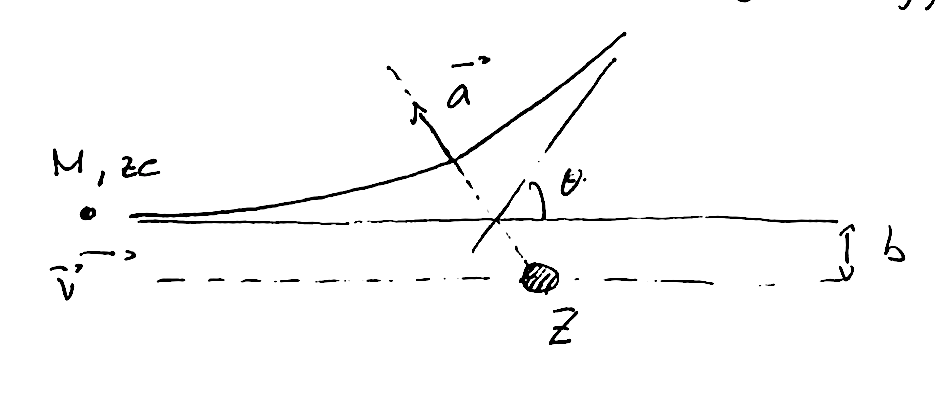
\includegraphics[width=0.6\textwidth]{passRadMat16}
  \caption{Illustration of the scattering of a charged particle by the Coulomb potential of a nucleus. 
  The moving scattered particle has a mass $M$, a charge $ze$ and a velocity $v$, while the nucleus has charge $Ze$ and the scattering angle is denoted as $\theta$; $b$ is the impact parameter. The nucleus produces an electric field which ``brakes'' the particle in motion and deviates its trajectory.
  }
\item{}
  \label{fig:passRadMat16}
\end{figure}

In the reference frame of the particle, the electric field is widened
by a factor $\gamma$ in the transverse direction as illustrated in Figure~\ref{fig:FieldBetheBloch}. Let us
consider a nucleus of charge $Ze$ and an incoming particle with charge
$ze$, mass $M$, velocity $v$ and with an impact parameter $b$ (see
figure \ref{fig:passRadMat16}). At the point of minimum distance the acceleration along the direction of motion vanishes, and the velocity is orthogonal to the particle-nucleus direction. We can write the first principle of dynamics in the reference frame of the moving particle as
\[a' = \frac{\gamma}{M} \frac{zZe^2}{4\pi\epsilon_0 r^2},\] 
where we introduced the $\gamma$ factor as an approximation for the averaged effect of the force on the probe particle in the region where it is closest to the nucleus.

In classical electrodynamics the radiated power is calculated as\footnote{See §14.2 from Ref.~\cite{jackson} - page 664.}
\begin{eqnarray}
\label{eq:AcceleratedChargePower}
  W' &=&  \frac{\rr{ze}^2}{6\pi\epsilon_0} \frac{a'^2}{c^3} \nonumber \\
     &=& \gamma^2 \frac{2}{3} \frac{z^4 Z^2 e^6}{\rr{4\pi\epsilon_0}^3}\frac{1}{r^4 M^2 c^3}.
\end{eqnarray}

The scattering time will then be  equal to
$2r/\gamma v$, which is the time during which the particle (in its rest frame) "feels" effectively the Coulomb potential and therefore the time is shorten by the length contraction due to the velocity of the nucleus in the probe particle's rest frame. The  energy emitted during this time $2r/\gamma v$ can then be calculated as
\begin{eqnarray*}
  \Delta E' &=& \int W' dt' \\
            &=& \gamma \frac{4}{3} \frac{z^4 Z^2 e^6}{\rr{4\pi\epsilon_0}^3} \frac{1}{r^3 M^2 c^3 v}.
\end{eqnarray*}

The frequency of this phenomenon is $\omega'_c = \gamma v/2r$, and so the emission frequency spectrum is
\[\frac{dE'}{d\omega'} \sim \frac{\Delta E'}{\omega'_c} = \frac{8}{3}
  \frac{z^4Z^2e^6}{\rr{4\pi\epsilon_0}^3}\frac{1}{r^2 M^2 c^3 v^2}\]
Since energy and frequency are linked by a constant, the frequency
spectrum is Lorentz--invariant. (The same argument does not apply for
the angle of emission of the radiation, but in the relativistic limit
the bremsstrahlung is emitted at $\theta \simeq 0$ and is independent
on the frequency.) This allows us to use the same formula in the
laboratory reference frame, which can be written in terms of the classical electron radius $r_e$ and of the fine structure constant $\alpha$ as
\[\frac{dE}{d\omega} = \frac{8}{3}r_e^2
  \frac{z^4Z^2e^2}{4\pi\epsilon_0}\frac{m_e^2}{M^2}\frac{1}{r^2
    \beta^2 c} = \frac{8}{3}r_e^2
  z^4Z^2(\hslash\alpha)\frac{m_e^2}{M^2}\frac{1}{r^2
    \beta^2}.\]
Energy is radiated as photons, and we can calculate the number of radiated photons  with energy $E_{\gamma}$:
since $E_\gamma = \hslash \omega$, one has
\[ dn (E_{\gamma}) = \frac{1}{E_\gamma} dE(E_\gamma),\]
which can be written in terms of energy spectrum $\der{E}{E_{\gamma}}$ as follows (be careful: this should not be seen as a simple derivative, but is the spectrum in bins of energies that is divided by the emitted energy to get the number of emitted photons):
\[ \der{n (E_{\gamma}) }{E_{\gamma}} = \frac{1}{E_\gamma} \der{E}{\hslash \omega}. \]

We want to calculate the number of radiated photons per unit of length of the path of the particle. Similarly to the case of Fig.~\ref{fig:passRadMat3}, we first need to evaluate the number of targets (i.e. nuclei) at reach for a given impact parameter $b\in\qq{b,b+db}$ and per unit of length $dl$, which is given by
\[\frac{\mathcal{N}_A\rho}{A} 2\pi b\,db\,dl.\]
From this, we get
\[\frac{d^2n}{dE_\gamma dl} = \frac{1}{E_\gamma}\frac{16\pi}{3} \frac{z^4}{\beta^2}r_e^2 \alpha \frac{m_e^2}{M^2} \frac{\mathcal{N}_AZ^2\rho}{A} \frac{b\ db}{r^2}.\]
If we assume that the distance at which the interaction takes place is $r = b$, we can integrate over $b$ and obtain
\[\frac{d^2n}{dE_\gamma dl} = \frac{1}{E_\gamma}\frac{16\pi}{3} \frac{z^4}{\beta^2}r_e^2 \alpha \frac{m_e^2}{M^2} \frac{\mathcal{N}_AZ^2\rho}{A} \ln\frac{b_{\max}}{b_{\min}}\]
In order to integrate this term over the photon energy, many non--trivial effects should be taken in consideration - in particular the shielding effect of the electrons in the atom.

As it was done for the energy loss by ionization, it is useful to define the energy loss in terms of the normalized path length $x$, where
\[x = \rho l\]
is expressed in \(\si{g/cm^2}\). The energy released by bremsstrahlung per unit length will then be
\[\frac{dE}{dx} = \int_0^E \frac{d^2n}{dE_\gamma dx} E_\gamma dE_\gamma.\]
In principle the energy is dependent on the impact parameter:  however, in this simplified (approximated) approach we will assume that the energy and the impact parameter are independent. As in the case of multiple scattering, one can take as integration limits for the impact parameter the approximated expression of the size of the nucleus and the size of the atom as a function of the atomic number, and obtain
\[\der{E}{x} = \frac{z^4}{\beta^2} \frac{m_e^2}{M^2}4r_e^2\alpha \frac{\mathcal{N}_AZ^2}{A}\ln\rr{183\ Z^{-\frac{1}{3}}}E\]

\subsection{Bremstrahlung for electrons}
For an {\bf electron} ($M = m_e$ and $z=1$), which in typical nuclear and particle physics experiments is a relativistic particle ($\beta \sim 1$), the energy loss can be expressed in terms of the radiation length $X_0$ defined in Eq.~\ref{eq:x0} as
\[\frac{dE}{dx} \simeq \frac{E}{X_0}.\]
A more detailed computation,which takes into account the phenomenon of screening from the atomic electrons,  gives
\[\der{E}{x} = 4r_e^2\alpha \frac{\mathcal{N}_AZ^2}{A}\qq{\ln\rr{183\ Z^{-\frac{1}{3}}}+\frac{1}{18}}E.\]

\subsection{Critical Energy}
The \emph{critical energy} for a given particle in a material is the value of energy for which the energy loss by radiation equals the energy loss by  ionization.
For the electron, an empiric parameterisation of the critical energy is given by
\[ E_c=\frac{800}{Z+1.2} \si{MeV}.\]

\subsection{Interpretation and summary}
The radiated power via bremsstrahlung is proportional to the square of the acceleration, i.e. to the inverse square of the mass (because the Coulomb potential does not depend on the particle mass). Consequently, this phenomenon is more important for very light particles (the electron and its antiparticle, the positron), while for particles of higher mass the effect is appreciable only at high energies: this is illustrated by Fig. \ref{fig:passRadMat17}, which shows the energy loss by bremsstrahlung and ionisation for electrons and positrons. Above a  few $\mega\electronvolt$ the bremsstrahlung process dominates over ionisation: the energy threshold at which this happens is called \emph{critical energy}, and depends on the material.

We have seen that the energy loss is almost constant (if expressed as a function of the particle energy). This is not completely true because the bremsstrahlung scales with energy!

From Fig. \ref{fig:passRadMat17} one can also see how the ionisation term (which dominates at low energy) is different for electrons and positrons, as expected (the material is not made of anti--matter!). Other effects are present at low energies:
\begin{itemize}
\item M\o{}ller scattering: $e^-\ e^- \to e^-\ e^-$;
\item Bhabha scattering:  $e^+\ e^- \to e^+\ e^-$;
\item Positron annihilation in matter: $e^+\ e^- \to \gamma \ \gamma $.
\end{itemize}
  
\begin{figure}
  \centering 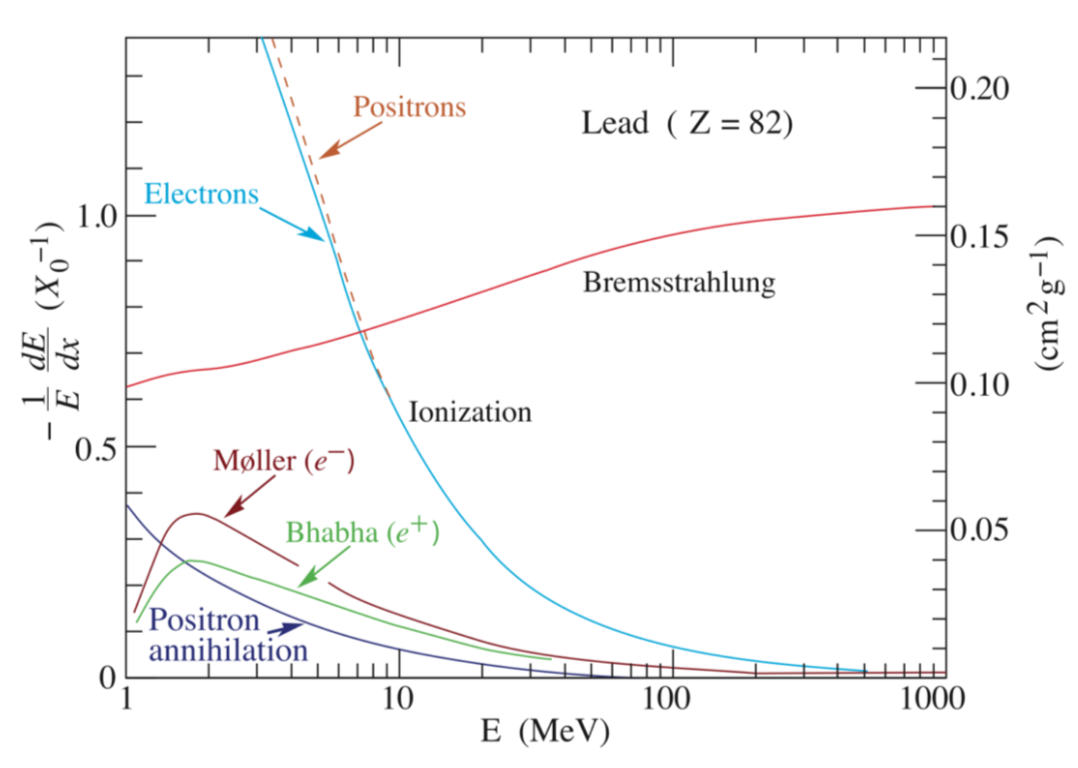
\includegraphics[width=\textwidth]{passRadMat17}
  \caption{Energy loss by bremsstrahlung and ionisation for electrons and positrons in a lead ($Z=82$) target, as a function of their energy. One can see how the ionisation term (which dominates at low energy) is different for electrons and positrons.
  The critical energy for electrons in typical materials is $\sim 10\,\mega\electronvolt$.
  Additional effects which give minor contributions to the energy loss (M\o{}ller scattering, Bhabha scattering and positron annihilation) are also shown.}
\item{}
  \label{fig:passRadMat17}
\end{figure}

\section{Interactions of Photons in Matter}\label{sec:IntPhotonsMatter}
\subsection{Photoelectric effect}
For photons with energy between the ionisation energy for the material and E$\sim 100\,\kilo\electronvolt$ the dominant interaction is photoelectric effect.

The interaction happens between a photon and an electron which is still bound to the atom. A similar interaction between a free electron and a photon can not happen due to the conservation of energy and momentum. In fact, if we denote the photon and electron energy and momentum as $E$, $E_e$ and $\vec{p}$, $\vec{p_e}$, respectively  (see Fig. \ref{fig:passRadMat18}), the conservation of the four-momentum norm can be written as
\begin{figure}
  \centering 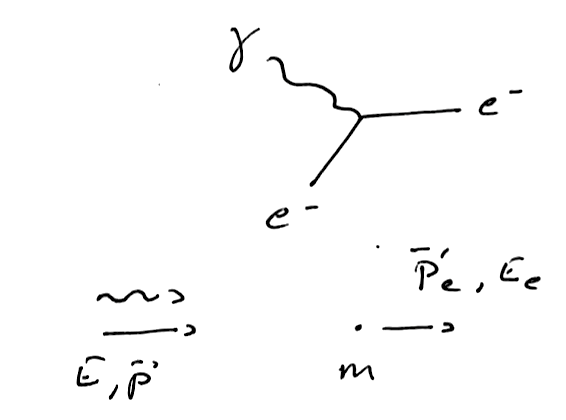
\includegraphics[width=0.5\textwidth]{passRadMat18}
  \caption{Illustration of the interaction between a photon and an atomic electron and the photoelectric effect. This simple diagram cannot take place alone due to energy and momentum conservation: what really happens is that the photon interacts with the atom as a whole.}
\item{}
  \label{fig:passRadMat18}
\end{figure}

\begin{eqnarray*}
  \rr{E+m,\vec{p}}^2 &=& \rr{E_e, \vec{p_e}}^2,\\
  E^2 + m^2 +2Em -p^2 &=& m^2,\\
  Em &=& 0,
\end{eqnarray*}
which is impossible.

The complete reaction for photoelectric effect is therefore
\[\gamma\ A \to A^+\ e^-.\]
If $E_l$ is the binding energy of the atom, electrons are emitted with energy
\[T = E_\gamma - E_l.\]
The cross section for this process is very small at high energy and grows when the photon energy approaches the binding energy of the $K$, $L$, $M\dots$ shells. Calculating the cross section of this process is hard, because the wave functions of the atomic electrons are complex to write -- although, for photon energies above the binding energy of the $K$ shell it's mostly $K$ electrons which contribute. For $E_\gamma \ll m_e c^2$ the cross section can be approximated as
\[\sigma_{\text{ph}} \simeq k Z^5 \frac{1}{E_\gamma^3},\]
where $k$ is a constant which depends only on $r_e$, $\alpha$ and $m_ec^2$, i.e. does not depend on the material.

\begin{figure}
  \centering 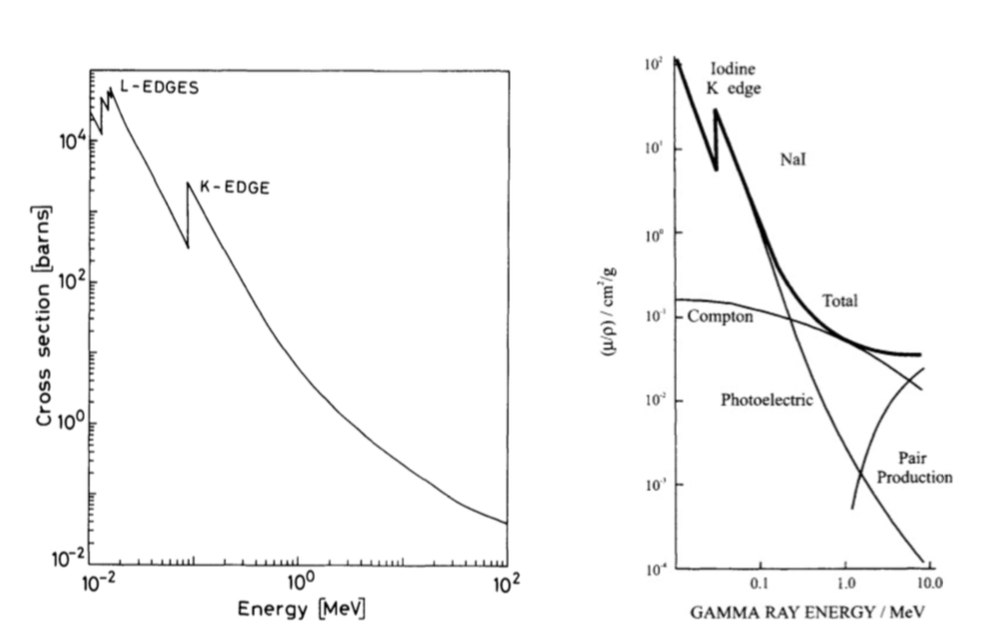
\includegraphics[width=\textwidth]{passRadMat17-5}
  \caption{Left: cross section of the photoelectric effect as a function of the photon energy $E_\gamma$. We can observe some peak near the energy of levels, which are due to the fact that electrons from more and more external shells start contributing when the photon energy is high enough. \\ Right: total photon interaction cross section as a function of $E_\gamma$ (bold line), with the individual contributions from photoelectric effect, Compton scattering and pair production.}
\item{}
  \label{fig:passRadMat17-5}
\end{figure}


\subsection{Compton effect}
When the photon energy is much greater than the binding energy of the electron, one can neglect the binding energy of the latter and consider atomic electrons as free particles. In this case, the dominant interaction is Compton scattering,
\[\gamma\ e^- \to \gamma\ e^-.\]

Let's compute the energy of the scattered photon, $E'$, in the reference frame of the initial electron of mass $m$, which is at rest (see figure \ref{fig:passRadMat19}).\\
\begin{figure}
  \centering 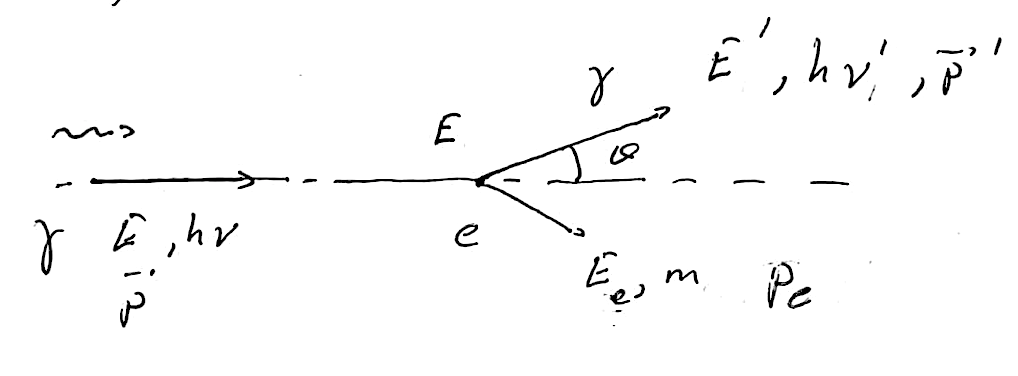
\includegraphics[width=0.5\textwidth]{passRadMat19}
  \caption{Illustration of the Compton effect: $\gamma$ is the photon with energy $h\nu$, $e$ is the electron at rest.
  After the collision the two particles scatter and in the picture we identify the scattering angle as $\theta$, i.e. the angle between the photon direction in the initial and final state. }
\item{}
  \label{fig:passRadMat19}
\end{figure}
We will use natural units in order to simplify notation, and denote with the subscript $e$ the electron quantities in the final state. The conservation of energy requires
\[E+m = E' + E_e,\]
while the conservation of momentum can be written as
\begin{eqnarray*}
  \vec{p} &=& \vec{p}'+\vec{p_e},\\
  \vec{p_e} &=& \vec{p} - \vec{p}'.
\end{eqnarray*}
We are interested in the photon energy in the final state, so we square the electron momentum with the goal of reducing the system of equations to one unknown:
\[p_e^2 = p^2 + p'^2 -2pp'\cos\theta,\]
while the energy-momentum equation for the electron can be written as
\[p_e^2 = E_e - m^2.\]
We use $E_e = E-E'+m$ and get
\begin{eqnarray*}
  \rr{E-E'+m}^2-m^2 &=& p^2 + p'^2 -2 pp'\cos\theta,\\
  2Em -2EE' -2E'm &=& -2EE'\cos\theta,\\
  E'\rr{E+m-E\cos\theta} &=& Em,
\end{eqnarray*}
which can be written as
\[E' = \frac{mE}{m+E-E\cos\theta}.\]
Finally, if we define $\epsilon = E/m$, we can write the photon energy in the final state as
\[E' = \frac{E}{1+\epsilon\rr{1-\cos\theta}}.\]
In agreement with intuition, the photon energy will be maximum for $\cos\theta = 1$ and minimum for $\cos\theta = -1$.

The energy released by the electron is
\begin{eqnarray*}
  \Delta E &=&  E-E'\\
           &=& h\nu - h\nu'\\
  &=& h\nu - \frac{h\nu}{1+\epsilon\rr{1-\cos\theta}}\\
  &=& \frac{h\nu\qq{1+\epsilon\rr{1-\cos\theta}}-h\nu}{1+\epsilon\rr{1-\cos\theta}},\\
  \Delta E &=& \frac{\epsilon h \nu \rr{1-\cos\theta}}{1+\epsilon\rr{1-\cos\theta}}.
\end{eqnarray*}
The maximum released energy corresponds to the minimum of $E'$, precisely:
\[\Delta E^{\max} = \frac{2 h \nu \epsilon}{1+2\epsilon} = h\nu \frac{2\epsilon}{1+2\epsilon}.\]
Reintroducing $c$, we come to the expression
\[\Delta E^{\max} = \frac{2\epsilon^2 m c^2}{1+2\epsilon},\]
which is called the \emph{Compton edge}.

The differential cross section for Compton scattering has been computed in 1928 by Klein and Nishina using quantum electrodynamics, and can be written as
\[\der{\sigma}{\Omega} = \frac{1}{2} r_e^2 \frac{Z}{A}\frac{E'}{E}\qq{1+\rr{\frac{E'}{E}}^2 + \rr{\frac{E'}{E}}\sin^2\theta}.\]
Keep in mind that the photon energy in the final state depends on the original photon energy and from the scattering angle, $E' = E'\rr{E,\theta}$. From this differential cross section one can compute (in a non-trivial way!) the high-energy limit of the total cross section for $E_\gamma\gg m_ec^2$,
\[\sigma_{\text{Compton}} \sim h\frac{Z}{A} \frac{8\pi r_e^2}{3}\frac{1}{E_\gamma},\]
and the low energy limit,
\[\sigma_{\text{Compton}} \sim h\frac{Z}{A} \frac{8\pi r_e^2}{3}\rr{1-2\frac{E_\gamma}{m_ec^2}}.\]

\begin{figure}
  \centering 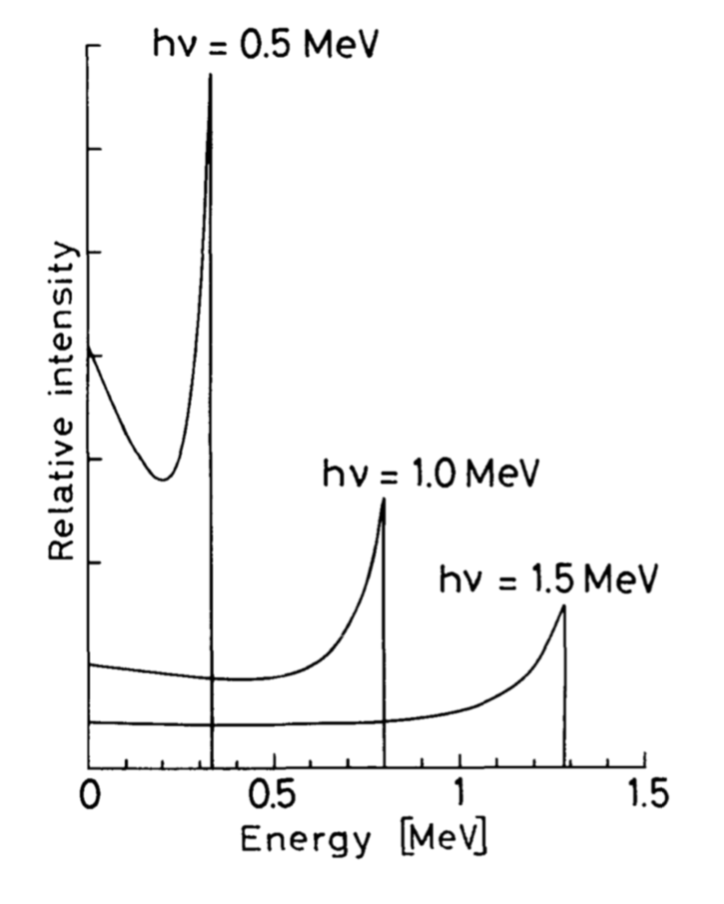
\includegraphics[width=0.5\textwidth]{passRadMat20}
  \caption{Distribution of the energy of electrons from Compton scattering, which illustrates the dependence of the Compton edge on the energy $h\nu$ of the incident photon. }
\item{}
  \label{fig:passRadMat20}
\end{figure}

\subsection{Classical Processes}
Two additional processes give minor contributions to the interaction of photons with matter, Thomson and Rayleigh scattering, which can be calculated using classical electrodynamics alone.

Thomson scattering corresponds to the electron--photon scattering when electrons can be considered as free and the photon energy is $E_\gamma \ll m_ec^2$. In this case the process, is modeled as an atomic electron which oscillates under the presence of an electromagnetic wave, emitting a secondary spherical wave.
The cross section for Thomson scattering is the following:
\[\sigma = Z\frac{8\pi}{3} r_e^2\]
and corresponds to the low energy limit of the Klein--Nishina formula.

In Rayleigh scattering, the whole atom takes part to the elastic scattering as a single object. For this reason this process is also called \emph{coherent scattering}.

While these two classical processes are important in atomic physics, they can be neglected when considering high-energy physics experiments, where usually -- for $E_\gamma\lesssim 2m_ec^2$ -- one takes into account only the photoelectric and Compton effects.

\subsection{Electron-Positron pair creation}
The creation of an electron--positron pair from a single photon would be
impossible in vacuum, because of four-momentum conservation. In order to
allow the process of \emph{pair production} by a photon, an external
electric field is needed. Of course, this process can happen in
presence of a nucleus (``recoil on a nucleus''),
\[\gamma\ N \to e^+\ e^-\ N,\]
or of another particle, like an atomic electron (``recoil on an electron''),
\[\gamma\ e^- \to e^+\ e^-\ e^-.\]
\begin{figure}
  \centering 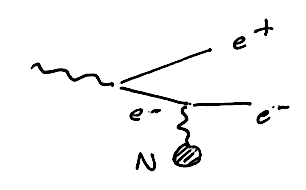
\includegraphics[width=0.5\textwidth]{passRadMat21}
  \caption{Illustration of the creation of an electron--positron pair in the presence of a nucleus $N$.}
\item{}
  \label{fig:passRadMat21}
\end{figure}

Pair production can only happen when the photon energy is above
$2m_ec^2$ (when the recoil is on a nucleus) or above $4m_ec^2$ (when the recoil is on an electron). In this second case the cross section is lower (see
Fig. \ref{fig:passRadMat22}).
\begin{figure}
  \centering 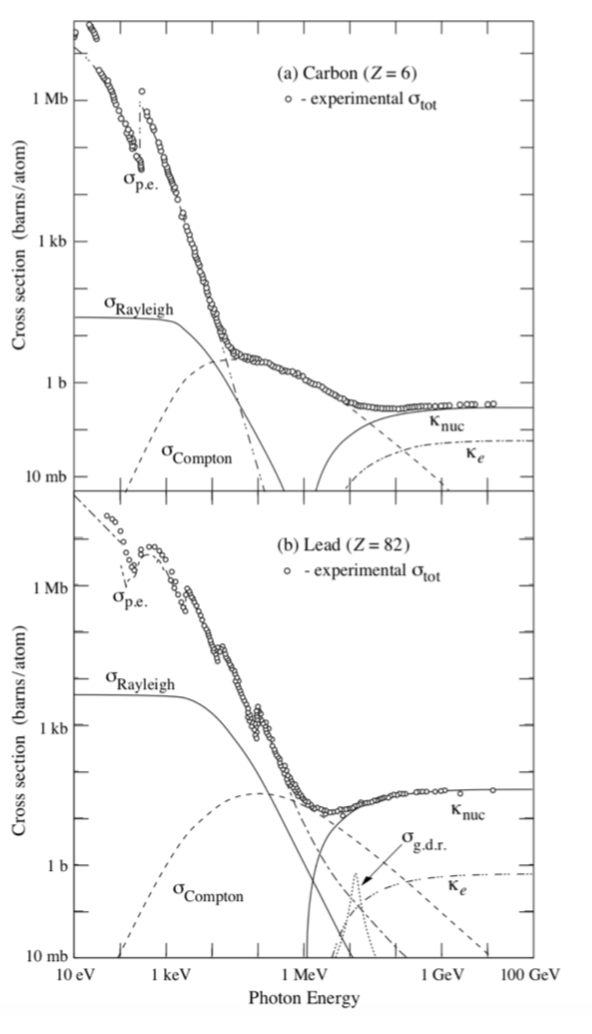
\includegraphics[width=\textwidth]{passRadMat22}
  \caption{Photon differential interaction cross sections in (a) carbon ($Z=6$) and (b) lead ($Z=82$), as a function of the probe photon energy. The agreement between the data and the prediction is clearly visible. The contributions to pair production in the presence of a nucleus or of an electron are denoted as $\kappa_\text{nuc}$ and $\kappa_e$, respectively.
  }
\item{}
  \label{fig:passRadMat22}
\end{figure}

As in the case of bremsstrahlung, pair production is screened at high energy,
which happens usually when $2m_ec^2 \ll E_\gamma \ll m_ec^2Z^{-1/3}/\alpha$. In this case, one has
\[\sigma_{\text{pair}} = \frac{Z^2}{137}r_e^2\rr{\frac{28}{9}\ln\frac{2E_\gamma}{m_ec^2}-\frac{218}{27}}.\]
When $E_\gamma \gg m_ec^2Z^{-1/3}/\alpha$, instead, the nucleus is screened and one has
\[\sigma_{\text{pair}} = \frac{Z^2}{137}r_e^2\rr{\frac{28}{9}\ln\frac{183}{Z^{\frac{1}{3}}}-\frac{2}{27}}.\]
Above the two--electron threshold the cross section rises sharply and when the nucleus appears to be screened it becomes constant.

At high energy one has
\[\sigma \propto Z,\]
and one can write
\[\sigma \sim \frac{7}{9} \frac{1}{X_0}\frac{A}{\mathcal{N}_A}\]
%It is important to notice the constant factor $\frac{7}{9}$ which will be found again in the calculation of mean free path.

\section{Electromagnetic showers}\label{sec:passRadMat_emShowers}
When they travel in a material, electrons and positrons  whose energy is above the critical energy (for electrons/positrons) of that material, or photons  whose energy is above the pair production  threshold, can start a cascade process which leads to the production of many electrons/positrons/photons in the material. This process is called \emph{electromagnetic shower} and is at the basis of the detection of these particles, with particle detectors called \emph{calorimeters}.\\

A schematic of this process is shown in Fig.
\ref{fig:passRadMat23}. Bremsstrahlung and pair production are the two
effects which dominate at high (electron/positron/photon) energy. A simplified model assumes that for
each travelled $X_0$, each photon converts into an electron--positron pair and
each electron/positron radiates a photon via bremsstrahlung. Under this approximation the
electromagnetic shower grows up, as long as the particle energy remains above the critical energy (as the pair
production threshold is usually lower than the critical energy).  Since the number of particles
doubles after one $X_0$, the number of particle after a distance $x$
(measured in terms of radiation lengths of the material, $X_0$) is
\[N = 2^x.\]
At each step, the energy held by the particle gets divided by
$2$, so one has
\[E_{N} = \frac{E_0}{2^x}.\]

Here are some values for the critical energy in different materials:

\begin{table}[h!]
\centering
  \begin{tabular}{ll}
    \hline
    Material & $E_c$                     \\ \hline
    Pb       & $5.5\  \mega\electronvolt$ \\
    Cu       & $24.8\  \mega\electronvolt$ \\
    Fe       & $27.4\  \mega\electronvolt$ \\
    Al       & $51.0\  \mega\electronvolt$ \\ \hline
  \end{tabular}
\end{table}

The maximum number of particles in the shower is reached after a
certain distance $x_{\max}$, for which the mean kinetic energy of the
particles will be equal to the critical energy,
\[\avg{E} = E_c \sim \frac{E}{2^x},\]
which gives
\[x_{\max}=\frac{\ln{\frac{E}{E_c}}}{\ln2}.\] For example, in the case of an electron of
$100\,\giga\electronvolt$, the maximum number of particles will be
reached for $x_{\max} \sim 13 X_0$, which for lead 
($X_0 \simeq 0.6\,\centi\meter$) corresponds to
$\sim 10\,\centi\meter$.

\begin{figure}
  \centering 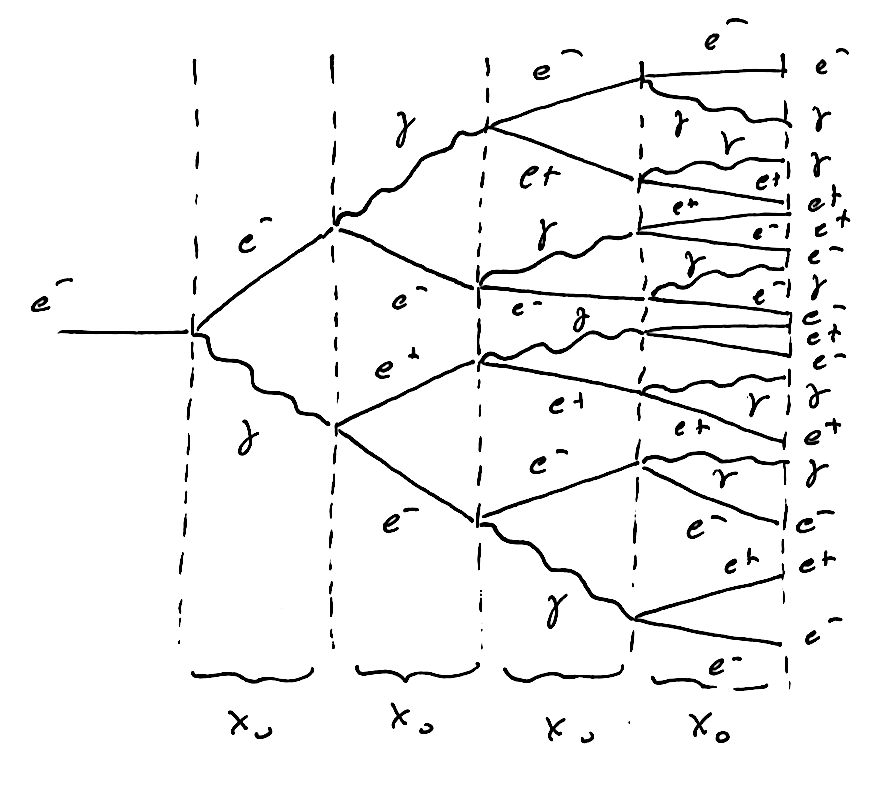
\includegraphics[width=0.6\textwidth]{passRadMat23}
  \caption{Schematic view of an electromagnetic shower.
  Here $X_0$ indicates the length of each interaction which causes a loss of energy, due to the splitting described in the text. The process ends (and the shower ``stops'') when the particle energy reaches $E<E_c$.}
  \label{fig:passRadMat23}
\end{figure}
